




%%%%%%%%%%%%%%%%%%%%%
\subsection{Lattices and Building Sets} 
\label{building-set-basics}
Although our results concern matroids, their lattices
of flats, building sets, and Chow rings, Feichtner and Yuzvinsky \cite{FY} actually worked at a higher level of generality: building sets in {\it atomic lattices} and their
Chow rings.  We start with this more general framework,
in order to present their integral Gr\"obner basis result.

Throughout, $\L$ will be a finite lattice, that is a finite poset in which any pair of elements $x,y$ has 
a least upper bound and greatest lower bound, called their join $x \vee y$ and meet $x \wedge y$.  Finiteness then implies than any subset $A \subseteq \L$ also has such 
a join $\vee A$ and meet $\wedge A$;  in particular,
the entire lattice
$\L$ itself has a top element $\hat{1}=\vee \L$ 
and bottom element $\hat{0}=\wedge \L$.  
For elements $F,F'$ in $\L$, the (closed) interval between them will be denoted $[F,F']:=\{ F'' \in \L: F \leq F'' \leq F'\}$.

\begin{defn} \cite[Def.~1]{FY}
    In a finite lattice $\L$, a subset $\G \subseteq \L \setminus \{\hat{0}\}$ is a \emph{building set} if for every $F$ in $\L \setminus \{\hat{0}\}$, letting
    $\max(\G_{\leq F})=\{F_1,\ldots,F_\ell\}$ denote the maximal elements of $\G_{\leq F}:=\{F' \in \G: F' \leq F\}$, one has  a poset isomorphism
    \[
        [\hat{0}, F] 
        \cong 
         [\hat{0},F_1] \times \cdots \times [\hat{0},F_\ell].
    \]
    On the right side, the Cartesian product of posets
    inherits a componentwise ordering from its factors.
\end{defn}

\begin{example}
The \emph{maximal building set} $\G_{\max}:=\L \setminus \{\hat{0}\}$ vacuously satisfies the conditions for a building set, as one always has $\max (\G_{\max})_{\leq F}=\{F\}$. 
At the other extreme, the \emph{minimal building set} $\G_{\min}$ is the set of {\it indecomposable} elements: those whose lower interval $[\hat{0}, F]$ cannot be decomposed as a nontrivial product.

 Note that the {\it atoms} of the lattice, which are
 the elements covering $\hat{0}$, are always indecomposable, and hence included in every building set.
\end{example}


%%%%%
\subsection{Nested sets}
\label{nested-set-subsection}
Each building set $\G \subseteq \L \setminus \{\hat{0}\}$ gives rise to a family of subsets of $\G$
called $\G$-\emph{nested sets}.

\begin{defn}\label{def:nested-sets}
    A subset $N \subset \G$
    is called $\G$-\emph{nested} if 
    for any pairwise incomparable $F_1, F_2, \ldots, F_t \in N$, their join $F_1\vee F_2\vee \cdots \vee F_t$ is not in $\G$. 
    Denote by $\N(\L,\G)$ the collection
    of all $\G$-nested sets.
\end{defn}

Note that $\N(\L,\G)$ is closed under
inclusion, forming an abstract simplicial
complex on vertex set $\G$. In general, every totally ordered subset $N \subset \G$ is vacuously $\G$-nested. 

\begin{example}
When $\G = \G_{\max}$, the $\G$-nested sets are the {\it chains} (=linearly ordered subsets) of $\L \setminus \{\hat{0}\}$. The collection of nested sets, $\N(\L,\G_{\max})$, forms the {\it order complex} for the poset $\L \setminus \{\hat{0}\}$.
\end{example}

\begin{example}
\label{partition-lattice-example}
    Let $\L= \Pi_n$, the {\it lattice of set partitions} of $\{1,2,\ldots,n\}$. 
    The indecomposable elements of this lattice are those set partitions having at most one non-singleton block. After removing the decomposable elements, the remaining lattice now has the Petersen graph as its underlying graph.
    The lattice $\L=\Pi_4$ is displayed on the left below.  The indecomposable elements are in black, and the decomposables in gray.

\begin{figure}[h]  
\centering 
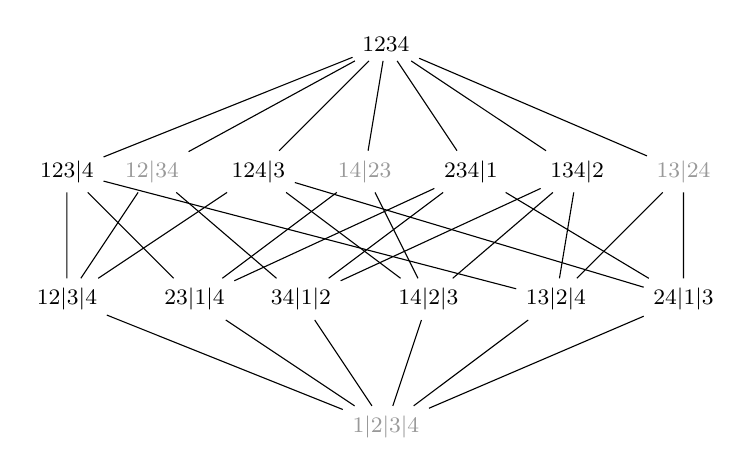
\begin{tikzpicture} [scale=.27,auto=left,every node]
   \node[gray!80] (0) at (10,-1) {\footnotesize $1\vert 2\vert 3\vert 4$};
  
  \node (1) at (-5,5) {\footnotesize $12\vert 3\vert 4$};
  \node (2) at (1,5) {\footnotesize $ 23\vert1\vert 4$};
  \node (3) at (6,5) {\footnotesize $34\vert 1\vert 2$};
  \node (4) at (12,5) {\footnotesize $14\vert 2\vert 3$};
  \node (5) at (18,5) {\footnotesize $13\vert 2\vert 4$};
  \node (6) at (24,5) {\footnotesize $24 \vert 1\vert 3$};
  
  \node (125) at (-5,11) {\footnotesize $123\vert 4$};
  \node[gray!80] (13) at (-1,11) {\footnotesize $12\vert 34$};
  \node (146) at (4,11) {\footnotesize $124\vert 3$};
  \node[gray!80] (24) at (9,11) {\footnotesize $14\vert 23$};
  \node (236) at (14,11) {\footnotesize $234\vert 1$};
  \node (345) at (19, 11) {\footnotesize $134\vert 2$};
  \node[gray!80] (56) at (24, 11) {\footnotesize $13\vert 24$};
  \node (e) at (10,17) {\footnotesize $1234$};
  \foreach \from/\to in {0/1,0/2,0/3, 0/4, 0/5, 0/6,
  1/125, 1/13,1/146, 
  2/125, 2/24, 2/236,
  3/13, 3/236, 3/345,
  4/146, 4/24, 4/345,
   5/125, 5/345, 5/56,
   6/146, 6/236, 6/56,
  e/125, e/13, e/146, e/24, e/56, e/345, e/236}
    \draw (\from) -- (\to);
\end{tikzpicture}
%\end{minipage}
%\begin{minipage}[h]{.2\textwidth}
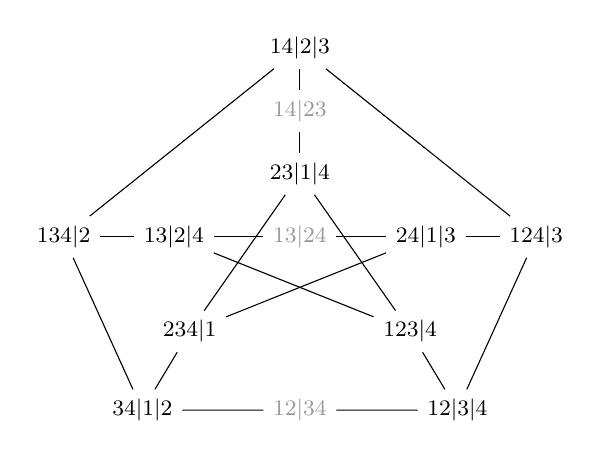
\begin{tikzpicture}
%[scale=.30,auto=left,every node/.style={circle,fill=black!15}]
 [scale=.20,auto=left,every node]
   \node[gray!80] (13-24) at (0,1) {\footnotesize $13|24$};
  \node (134) at (-15,1) {\footnotesize $134|2$};
  \node (13) at (-8,1) {\footnotesize $13|2|4$};
  \node (24) at (8,1) {\footnotesize $24|1|3$};
  \node (124) at (15,1) {\footnotesize $124|3$};
  \node (14) at (0,13) {\footnotesize $14|2|3$};
  \node[gray!80] (14-23) at (0,9) {\footnotesize $14|23$};
  \node (23) at (0,5) {\footnotesize $23|1|4$};
  \node (234) at (-7,-5) {\footnotesize $234|1$};
  \node (123) at (7,-5) {\footnotesize $123|4$};
  \node (34) at (-10,-10) {\footnotesize $34|1|2$};
  \node[gray!80] (12-34) at (0,-10) {\footnotesize $12|34$};
  \node (12) at (10,-10) {\footnotesize $12|3|4$};
  \foreach \from/\to in {134/13,13/13-24,13-24/24,24/124,134/14,14/124,124/12,12/12-34,12-34/34,34/134,34/234,234/24,14/14-23,14-23/23,23/234,23/123,13/123,12/123}
    \draw (\from) -- (\to);
\end{tikzpicture}
%\end{minipage}
\end{figure}


The nested set complexes $\N(\L,\G_{\max}), \N(\L,\G_{\min})$ are both two-dimensional simplicial complexes which are cones with
apex/cone vertex $1234$; the base of the cone is the one-dimensional complex on the right above in the case of $\N(\L,\G_{\max})$.  For  $\N(\L,\G_{\min})$, the base of the cone is obtained from the same picture by {\it unsubdividing}  three edges, removing the vertices that correspond to the
decomposables $12|34, 13|24, 14|23$:
\begin{align*}
34|1|2 - 12|34 - 12|3|4 &\quad  \rightsquigarrow \quad 34|1|2 - 12|3|4,\\
13|2|4 - 13|24 - 24|1|3 &\quad \rightsquigarrow \quad 13|2|4 - 24|1|3,\\
14|2|3 - 14|23 - 23|1|4 &\quad \rightsquigarrow \quad 14|2|3 - 23|1|4.\\
\end{align*}
In this $n=4$ case, the graph on the right above is homeomorphic to the {\it Petersen graph}; compare these figures with those in 
%Ardila and Klivans 
\cite[Fig.~2]{ArdilaKlivans}, %Feichtner and Sturmfels
\cite[Fig.~2]{FeichtnerSturmfels}, %Feichtner and Yuzvinsky 
\cite[p.~21]{FY}.  See also Example~\ref{ex:maximal-and-minimal-versus-hypotheses} for further discussion.
\end{example}

Interestingly, the restriction of the poset structure on $\L$ to any of its $\G$-nested sets $N$ becomes very simple.  Recall that a {\it forest poset} (as in, e.g., Bj\"orner and Wachs \cite{BjornerWachs}) is a finite poset in which each element is covered by at most one other element of the poset.  Note that this is {\it stronger} than simply requiring that the Hasse diagram of the poset is a forest, that is, an acyclic graph. 

\begin{lemma}\label{lem:rooted-forest}
 \cite[Prop.~2.4(4)]{PagariaPezzoli}
 For any building set $\G \subseteq \L \setminus \{\hat{0}\}$,
 the poset $\L|_N$ for any $\G$-nested set $N$ is always a forest poset.
 % that is, each element in $N$ is covered by at most one other element of $N$. 
 In particular, incomparable $F,F'$ in $N$ have disjoint principal ideals  $N_{\leq F}, N_{\leq F'}$, that is, $N_{\leq F} \cap N_{\leq F'}=\varnothing$.
\end{lemma}


\subsection{Atomic and geometric lattices and matroids}
\label{matroid-background-section}
So far these notions have played no role.  However,
atomicity is important in Feichtner and Yuzvinsky's  Gr\"obner basis presentation for their Chow ring $A(\L,\G)$, while the geometric lattice/matroid assumption implies a crucial numerical identity, Lemma~\ref{lem:crucial-numerical-fact} below.

\begin{defn}
Recall the {\it atoms} of a finite lattice $\L$ are
the elements that cover $\hat{0}$.  One calls $\L$ {\it atomic} if every $F$ in $L$ is the join of the set of atoms lying weakly below $F$ in $\L$.
\end{defn}

When $\L$ is a finite {\it atomic} lattice, the following quantity
%originally defined in \cite{FY},
is well-defined
for any $F,F'$ in $\L$ with $F \leq F'$:
\begin{equation}
\label{atomic-lattice-metric}
d(F,F')= \min \{d: F'=F \vee a_1 \vee \cdots \vee a_d \text{ for some atoms }a_1,\ldots,a_d \in \L\}.
\end{equation}
Well-definedness follows from the fact that
it is a minimum over a (finite) set of positive integers which is nonempty, as $F'=F \vee a_1 \vee \cdots \vee a_d$ where $\{a_1,\ldots,a_d\}$
is the set of {\it all} atoms of $L$ 
with $a_i \leq F'$.

This function $d(F,F')$ behaves more simply under extra
hypotheses on $\L$.

\begin{defn}
    A finite lattice $\L$ is {\it semimodular} if  $F,F'$ covering $F \wedge F'$ implies
    $F \vee F'$ covers $F, F'$.
\end{defn}

It is well-known \cite[Prop.~3.3.2]{Stanley-EC1} that, for a finite lattice $\L$, this condition is equivalent to being {\it ranked} and having the rank function $\rk: L \rightarrow \{0,1,2,\ldots\}$ obey the {\it semimodular inequality}
\begin{equation}
\label{semimodular-inequality}
\rk(F \vee F') + \rk(F \wedge F') \leq \rk(F)+\rk(F').
\end{equation}

\begin{defn}
    An atomic semimodular lattice $\L$ is called a {\it geometric lattice}.
\end{defn}
\noindent For geometric lattices $\L$, one can check that
the semimodular inequality \eqref{semimodular-inequality} implies this rewriting of \eqref{atomic-lattice-metric}:
\begin{equation}
\label{metric-rewritten}
d(F,F')=\rk(F')-\rk(F).
\end{equation}
\noindent
Finite geometric lattices are known \cite[\S3.3]{Stanley-EC1} to be the same as lattices of flats of finite {\it matroids}, briefly reviewed here. 
On matroids, some excellent references include Oxley \cite{oxley} and Ardila \cite{icm_matroids}.

\begin{defn} \label{flats} \rm
A matroid $\M = (\E, \L_\M)$ consists of a (finite) ground set $\E$ and a collection of subsets $\L_\M =\{F\} \subseteq 2^\E$ called {\it flats},
satisfying these axioms:
\begin{enumerate}
    \item[(F1)] $\E\in \L_\M$. %The ground set is a flat 
    \item[(F2)] If $F, F'\in \L_\M$ , then $F \cap F' \in \L_\M$. %The meet of two flats is a flat  
    \item[(F3)] For any $F\in \L_\M$, and any $i \in \E\setminus F$, there is a unique $F' \in \L_\M$ containing $i$ which {\it covers $F$} in this sense: 
    $F \subsetneq F'$, and no other flat $F''$ has $F \subsetneq F'' \subsetneq F'$. 
\end{enumerate} 
\end{defn}
These axioms combinatorially abstract properties of a {\it realizable matroid} $\M$ coming from a list of vectors $v_1,v_2,\ldots,v_n$
in a vector space over some field $\mathbb{F}$.  
A realizable matroid $\M$ has ground set $E=\{1,2,\ldots,n\}$, and $F \subseteq E$ is a flat in $\L_\M$ when 
the inclusion $F \subseteq 
 \{i \in E: v_i \in \spn_{\mathbb{F}}\{ v_j\}_{j \in F} 
 \}$ is an equality. 
Axioms (F1),(F2) imply that the inclusion poset 
on $\L_\M$ forms a lattice, with {\it meets} $F \wedge F'=F \cap F'$ and {\it joins}
$F \vee F'=\bigcap_{F'' \supseteq F,F'} F''$.
Axiom (F3) further implies that the lattice $\L_\M$ will be {\it geometric}.
The {\it rank} of the matroid $\M$ itself is defined to be $\rk(E)$, which we assume throughout has $\rk(E)=r+1$. 

\begin{remark}
In this paper, we will only consider {\it simple matroids}, that is, 
\begin{itemize}
    \item $\M$ is {\it loopless}, so that $\hat{0}=\bigcap_{F \in \L_\M} F =\varnothing$ is a flat, and 
    \item $\M$ has no {\it parallel elements}, so that the atoms of $\L_\M$ are all singleton flats $F=\{a\}$.
\end{itemize}
This means that $\M$ is completely determined by
the geometric lattice $\L=\L_\M$.  This does not
impose a serious restriction, since the Chow ring $A(\L,\G)$ defined in Section~\ref{Chow-ring-section} below only uses information about the lattice strucutre of 
$\L$ and the choice of
building set $\G \subseteq \L \setminus \{\hat{0}\}$.  
\end{remark}

 The matroid automorphisms $\Aut(\M)$ of $\M$ are the permutations $g$ of the ground set $E$ preserving $\L_\M$ setwise, that is, sending flats $F$ to flats $g(F)$.  These also give poset and
lattice automorphisms of $\L_\M$. For a subgroup $\subgroup \subseteq \Aut(\M)$, a building set $\G$ is called \textit{$\subgroup$-stable} if each $g \in \subgroup$ preserves $\G$ setwise.

\begin{example}
\label{ex:maximal-and-minimal-versus-hypotheses}
For any $\subgroup \subseteq \Aut(\M)$, the maximal and minimal building sets 
$\G_{\max}, \G_{\min}$ are both $\subgroup$-stable.  
On the other hand, Theorem~\ref{main-theorem} imposes two extra technical conditions, the first being that the building set contains the ground set $E=\hat{1}$.
This always holds for $\G_{\max}$.  It holds for $\G_{\min}$ if and only if $\L=\L_\M$ for a {\it connected} (simple) matroid $\M$, that is, one cannot express $\M = \M_1 \oplus \M_2$ as a nontrivial direct sum.  

The second technical condition is the
stabilizer condition \eqref{eq:stabilizer-condition}, saying that a nested set which is setwise stabilized by some 
$g$ in $G$ must also be pointwise stabilized.  Again this always holds for $\G_{\max}$.  However for $\G_{\min}$, this condition can easily fail.  One such example of this type is the Chow ring for the {\it moduli space $\overline{M}_{0,n+1}$ of genus $0$ curves with $n+1$ marked points}; see, e.g., Dotsenko \cite{dotsenko}, Gibney and Maclagan \cite{GibneyMaclagan},  Keel \cite{Keel}, Maestroni and McCullough \cite[Rmk.~2.4]{MaestroniMcCullough}. This Chow ring turns out to be
$A(\L_\M,\G_{\min})$ where $\M$ is the graphic matroid associated to a complete graph on $n$ vertices and $\L_\M=\Pi_n$ is the set partition lattice from Example~\ref{partition-lattice-example}. In Remark~\ref{rmk:conclusion-failure} below, we explain how both the stabilizer condition \eqref{eq:stabilizer-condition} and the conclusion of Theorem~\ref{main-theorem} fail for this Chow ring when $n=12$.

% To see an example of where the stabilizer condition \eqref{eq:stabilizer-condition} fails, consider $\L_\M = \Pi_{12}$, with $G=\Aut(M)$ being the symmetric group $\symm_{12}$. Then consider the nested set 
%     \begin{align*}
%     N = \{F_1, F_2, F_3\}, \text{ where } F_1 &= 1,2,3,4|5|6|7|8|9|10|11|12, \\
%     F_2 &= 5,6,7,8|1|2|3|4|9|10|11|12, \\ 
%     \text{ and } F_3 &= 9,10,11,12|1|2|3|4|5|6|7|8.
%     \end{align*}
% The set $N$ is nested because the join $F_1 \vee F_2 \vee F_3 = 1,2,3,4|5,6,7,8|9,10,11,12$ has multiple non-singleton blocks, and is therefore not a member of $\G_{\min}$. The permutation $g = (1,5,9)(2,6,10)(3,7,11)(4,8,12)$ in $\symm_{12}$, expressed here in cycle notation, fixes $N$ setwise, but not pointwise:
% it sends $F_1 \mapsto F_2 \mapsto F_3 \mapsto F_1$.


\end{example}


\subsection{A surprisingly important identity} \label{suprising-identity-section}
A certain quantity from
Feichtner and Yuzvinsky \cite[\S3]{FY},
controls their 
Gr\"obner bases: for 
an atomic lattice $\L$, building set $\G$, and $\G$-nested set $N$ with $F \in N$, define
\begin{equation}
\label{atomic-version-of-crucial-quantity}
m_N(F):=d(\vee N_{<F},F)
\end{equation}
where $N_{<F}:=\{F' \in N: F' < F\}$.
For geometric lattices, \eqref{metric-rewritten} lets one rewrite \eqref{atomic-version-of-crucial-quantity} as in the Introduction:
\begin{equation}
\label{crucial-quantity}
m_N(F):=\rk(F) - \rk \left( \vee N_{<F} \right).
\end{equation}

The next identity involving $m_N(F)$ for geometric lattices plays a surprisingly crucial role here.
It appears in the proof of Corollary~\ref{Chow-ring-degrees} bounding the degrees occurring in a Chow ring.
It similarly appears in the proof of Theorem~\ref{main-theorem},
showing certain subsets of FY-monomials, forming products of chains under divisibility, live in intervals of degrees {\it symmetrically placed} with respect to the grading on
the Chow ring $A(\M,\G)$.

\begin{lemma}\label{lem:crucial-numerical-fact}
For any geometric lattice $\L$, any building set $\G$,
and any $\G$-nested set $N$, its join 
$\vee N$ has its rank expressible as
$
  \rk(\vee N)= \sum_{F \in N} m_N(F).
$
\end{lemma}

\begin{proof}
Proceed by induction on $|N|$.  The base case $N=\varnothing$ has $\rk(\vee N)=\rk(\hat{0})=0$ equal to the empty sum.
In the inductive step, let the set of inclusion-maximal elements
$\max(N)=\{F_1,\ldots,F_\ell\}$ 
have size $\ell$, and proceed by cases $\ell=1$
versus $\ell \geq 2$.

\vskip.1in
\noindent
{\sf Case 1.} $\ell=1$.

Here $F_1=\vee N$.
Letting $\hat{N}$ denote the $\G$-nested set $N \setminus \{F_1\}$, one has this calculation:
$$
\sum_{F \in N} m_N(F)
= m_N(F_1) + \sum_{F \in \hat{N}} m_N(F)
= m_N(F_1) + \sum_{F \in \hat{N}} m_{\hat{N}}(F) 
\overset{(*)}{=} m_N(F_1)+ \rk(\vee \hat{N}) 
=\rk(F_1)=\rk(\vee N)
$$
where equality (*) applied the inductive hypothesis to the nested set $\hat{N}$.


\vskip.1in
\noindent
{\sf Case 2.} $\ell \geq 2$.

From \cite[Prop 2.8]{FK}, one has that 
$
\max\G_{\leq \vee N} = \{F_1, F_2, \ldots, F_\ell\},
$
and therefore
$[\hat{0},\vee N] \cong \prod_{i=1}^\ell [\hat{0},F_i]$.
This gives the first equality in the following
calculation, whose remaining equalities are justified below:
\begin{align*}
\rk(\vee N) 
    = \sum_{i=1}^\ell \rk(F_i) 
    \overset{(**)}{=} \sum_{i=1}^\ell  \sum_{F \in N_{\leq F_i}} m_{N_{\leq F_i}}(F)  
    = \sum_{i=1}^\ell \sum_{F \in N_{\leq F_i}} m_N(F) 
    \overset{(***)}{=} \sum_{F \in N} m_N(F) 
\end{align*}
Equality (**) used the assumption $\ell \geq 2$, to apply the inductive hypothesis to each $\G$-nested set $N_{\leq F_i}$. Equality (***) used the fact that one has a disjoint decomposition
$N=\sqcup_{i=1}^\ell N_{\leq F_i}$
by Lemma~\ref{lem:rooted-forest}.
\end{proof}



\begin{comment}
\begin{proof}
Suppose, for the sake of contradiction, that there exist flats $F_1, F_2, F_3 \in N$ such that 
\[F_3 < F_1, \quad F_3 < F_2 \quad \text{and} \quad F_1, F_2 \text{ are incomparable.}\]
Since a subset of a nested set is also nested, we know that $\{F_1, F_2\}$ is a nested set. By lemma~\ref{antichain}, it follows that the rank $\rk(F_1 \vee F_2)$ is the sum of the flats' individual ranks $\rk(F_1)+\rk(F_2)$.

The lattice of flats is upper semimodular, meaning that
\[\rk(F_1 \wedge F_2) + \rk(F_1 \vee F_2) \leq \rk(F_1)+\rk(F_2),\] 
hence making $F_1 \wedge F_2 = \varnothing$. 
Since $F_3 < F_1$ and $F_3 < F_2$, 
we have $F_3 \leq (F_1 \wedge F_2) = \varnothing,$ so $F_3 = \varnothing$. However, every nested set is a subset of some building set, which exclude the empty flat by definition.
\end{proof}
\end{comment}








%%%%%%%%%%%%%%%%%%%%%
\subsection{Chow Rings}
\label{Chow-ring-section}
The following definition was introduced by
Feichtner and Yuzvinsky \cite{FY}.


\begin{defn} 
\label{Chow-ring-definition}
For a finite lattice $\L$ and building set $\G$, 
the \emph{Chow ring} $A(\L, \G)$ is the quotient $\Z$-algebra 
    $$
    A(\L, \G) := S/(I+J)
    $$
    where $S=\Z[x_F]_{F \in \G}$ is a polynomial algebra, and $I,J$ are the following ideals of $S$:
    \begin{itemize}
      \item $I$ is the {\it Stanley-Reisner ideal} for the simplicial complex $\N(\L,\G)$, meaning it is
      generated by products $x_{F_1} x_{F_2} \cdots x_{F_t}$ for subsets  $\{F_1, F_2, \ldots, F_t\} \subset \G$ which are {\it not} $\G$-nested.
    \item $J$ is generated by the linear elements
$\displaystyle\sum_{a \in F \in \G} x_F$ for each atom $a$ 
%(= element of rank $1$) 
in $\L$.
    \end{itemize}
\end{defn}

We wish to consider subgroups $\subgroup$ of the group $\Aut(\L)$ of poset automorphisms of $\L$, and building sets $\G \subseteq \L \setminus \{\hat{0}\}$ setwise stabilized by $\subgroup$, meaning $g(F) \in \G$ for all $F \in \G$ and $g$ in $\subgroup$.  We claim that in this setting, any $g$ in $\subgroup$ also acts by a $\Z$-algebra automorphism on $A(\L,\G)$ via $g(x_F)=x_{g(F)}$;  the key points are that poset automorphisms $g$ of $\L$
\begin{itemize}
\item preserve order and carry atoms to atoms, thus sending generators of $J$ to other generators of $J$, and 
\item because they
are also lattice automorphisms, they carry $\G$-nested sets to $\G$-nested sets, thus sending generators of $I$ to other generators of $I$.
\end{itemize}

We will also wish to consider $A(\L,\G)$ as a {\it graded} $\Z$-algebra, in which it inherits the standard grading on
$S=\Z[x_F]_{F \in \G}$ for which each variable $x_F$ has
$\deg(x_F)=1$.  This happens because the ideals $I,J \subset S$ are both graded ideals, generated by homogeneous elements of $S$. Also, subgroups $\subgroup \subset \Aut(\L)$ act as above via graded $\Z$-algebra automorphisms, that is, 
$A(\L,\G)=\bigoplus_{k=0}^\infty A^k$
and each $A^k$ becomes a $\Z \subgroup$-module.


\begin{comment}
\begin{remark}
\begin{itemize}
    \item $A(\L, \G)$ depends
only upon the associated {\it simple matroid} of $\M$.  That is,
one may assume $\M$ has
\begin{itemize}
    \item  no {\it loops}, meaning that one has empty 
intersection  $\varnothing = \bigcap_{F \in \L_\M} F$, and
\end{itemize}
Thus without loss of generality,
one may assume that $\M$ is a simple matroid throughout.
\end{itemize}
\end{remark}
\end{comment}



It is not yet clear that $A(\L, \G)$ has only
finitely many non-vanishing components $A^k$.
For this, we next 
consider Feichtner and Yuzvinsky's remarkable Gr\"obner basis presentation
mentioned in the Introduction.

\subsection{In praise of the Feichtner--Yuzvinsky Gr\"obner basis}

We recall here a version of Gr\"obner basis theory with respect to monomial orders on polynomial rings 
$
\Z[\xx]:=\Z[x_1,\ldots,x_n]
$
over $\Z$, used in \cite{FY}.

\begin{defn}\rm
A linear order $\prec$ on the set of all monomials $\{ \xx^\alpha:=x_1^{\alpha_1} \cdots x_n^{\alpha_n}\}$ in $\Z[\xx]$ is called a {\it monomial ordering}
if it is a {\it well-ordering} (every subset of monomials has a $\prec$-minimum element) and $\xx^\alpha \prec \xx^\beta$ implies
$\xx^\alpha \cdot \xx^\gamma \prec \xx^\beta \cdot \xx^\gamma$
for all $\alpha,\beta,\gamma$ in $\{0,1,2,\ldots\}^n$.
\end{defn}

\begin{example} \rm
After fixing a linear order on the variables $x_1 < \cdots < x_n$,
the associated {\it lexicographic order} $\prec$ has
$\xx^\alpha \prec \xx^\beta$ if there exists some $k=1,2,\ldots,n$ with  $\alpha_1 = \beta_1, \alpha_2=\beta_2,\ldots,\alpha_{k-1} = \beta_{k-1}$,
but $\alpha_k < \beta_k$.
\end{example}

\begin{defn}\rm
For $f=\sum_\alpha c_\alpha \xx^\alpha$ in $\Z[x_1,\ldots,x_n]$,
let $\init_\prec(f)=\xx^\beta$ denote the $\prec$-largest monomial in $f$ having $c_\beta \neq 0$.  Say $f$ is {\it $\prec$-monic} if the initial monomial $\init_\prec(f)=\xx^\beta$ has its coefficient $c_\beta=\pm 1$.

Having fixed a monomial order $\prec$, for any ideal $I \subset \Z[\xx]$, one says that a subset  $\{g_1,\ldots,g_t\} \subset I$ is a {\it monic Gr\"obner basis} for $I$ (with respect to $\prec$) if each $g_i$ is $\prec$-monic, and 
every $f$ in $I$ has $\init_\prec(f)$ divisible by at least one
of the intial monomials 
$\{ \init_\prec(g_1),\ldots,\init_\prec(g_t)\}$.
One calls $\xx^\alpha$ a {\it standard monomial} for 
$\{g_1,\ldots,g_t\}$ with respect to $\prec$ if
$\xx^\alpha$  is divisible by none of $\{ \init_\prec(g_1),\ldots,\init_\prec(g_t)\}$.
\end{defn}

It should be noted that some ideals $I \subset \Z[\xx]$
have {\it no} monic Gr\"obner basis, e.g. $I=(2) \subset \Z[x]$.  However, whenever $I$ {\it does} have a monic Gr\"obner basis, it has the following strong consequence, proven exactly as for Gr\"obner bases over
$\mathbb{F}[\xx]$ with field cofficients $\mathbb{F}$; see, e.g.,
Cox, Little, O'Shea \cite[\S2.5, 5.3]{CLO}.
\begin{prop}
\label{GB-basis-fact}
Given a monic Gr\"obner basis $\{g_1,\ldots,g_t\}$ for $I \subset S=\Z[\xx]$ with respect to $\prec$, then
\begin{itemize}
\item $I=(g_1,\ldots,g_t)$, that is, $\{g_1,\ldots,g_t\}$ generate $I$ as an ideal.
\item The quotient ring $S/I$ is a free $\Z$-module, with
a $\Z$-basis given by the standard monomials $\{x^\alpha\}$.
\end{itemize}
\end{prop}

The following crucial result appears as \cite[Thm. 2]{FY}.  To state it, define an {\it FY-monomial order} on $S=\Z[x_F]_{F \in \G}$ to be any monomial order
based on a linear order of the variables with $x_F > x_{F'}$ if $F < F'$.

\begin{thm}
\label{FY-GB-theorem}
Let $\L$ be a finite atomic lattice, and $\G \subset \L \setminus \{\hat{0}\}$ a building set.
Then for any choice of an $\FY$-monomial order on the ring $S=\Z[x_F]_{F\in \G}$,
the ideal $I+J$ presenting  $A(\L, \G)=S/(I+J)$
has a monic Gr\"obner basis consisting of the following
elements, along with their $\prec$-initial terms:
\begin{itemize}
\item
all $x_{F_1} x_{F_2} \cdots x_{F_t}$ for sets $\{F_1,F_2,\ldots,F_t\} \subset \G$ which are {\it not} $\G$-nested, each its own $\prec$-initial term,
\item 
for each $\G$-nested set $N$ with maximal elements
$\{F_1,\ldots,F_\ell\}$, and for each $F$ in $\G$ with $F > \vee N$,
\begin{align*}
\text{ the product }\quad x_{F_1} \cdots x_{F_\ell} 
&\left( \sum_{F' \geq F} x_{F'} \right)^
{d(\vee N, F)}\\
\text{ whose $\prec$-initial term is }\quad  
x_{F_1} \cdots x_{F_\ell} \cdot  &x_F^
{d(\vee N, F)}.
\end{align*}
\end{itemize}
\end{thm}

This has the following very strong consequence,
using the notation $m_N(F):=d(\vee N_{<F}, F)$ defined in \eqref{atomic-version-of-crucial-quantity}, where
$d(F,F')=\min\{d:F'=F \vee a_1 \vee \cdots \vee a_d \text{ for atoms }a_i \in \L\}$ was
defined in \eqref{atomic-lattice-metric}.


\begin{cor} (\cite[Cor. 1]{FY}) 
\label{cor: mon_basis}
Under the hypotheses of Theorem~\ref{FY-GB-theorem},
the Chow ring $A(\L,\G)$ is free as a $\Z$-module, with
the $\prec$-standard monomial $\Z$-basis given by the set of $\FY$-monomials
\begin{equation}
\label{FY-monomials-definition}
\fy := \left\{ x_{F_1}^{m_1} \cdots x_{F_\ell}^{m_\ell}: 
N=\{F_1,\ldots,F_\ell\} \text{ is }\G\text{-nested, and }0 \leq m_i <m_N(F_i)\right\}.
\end{equation}
\end{cor}

This has a particularly interesting further consequence for symmetries of $\L$,
inspired by work of H.-C. Liao on the Chow rings of Boolean lattices $\L$
with their maximal building set $\G_{\max}$; see \cite[Thm. 3.6]{Liao_new}.

\begin{cor}
\label{Chow-ring-carries-perm-reps-cor}
Under the hypotheses of Theorem~\ref{FY-GB-theorem},
if one has a subgroup $\subgroup \subseteq
\Aut(\L)$ setwise stabilizing the
building set $\G$, then
$\subgroup$ permutes the set $\FY$,
as well as its subset of degree $k$ monomials $\FY^k \subset \FY$.  

Consequently, the $\Z \subgroup$-modules on the Chow ring $A(\L, \G)$ and each of its homogeneous components $A^k$ lift to $\subgroup$-permutation representations on $\FY$ and each $\FY^k$.  
\end{cor}
\begin{proof}
It was noted that $g$ in $\subgroup$ sends $\G$-nested sets $N$ to
$\G$-nested sets $g(N)$.  Since such $g$ are lattice automorphisms, they have $g(\vee N)=\vee g(N)$.  Also $d(g(F),g(F'))=d(F,F')$, so that
$m_{g(N)}(g(F))=m_N(F)$.
Thus $g$ sends $\fy$-monomials
$x_{F_1}^{m_1} \cdots x_{F_\ell}^{m_\ell}$
to other $\fy$-monomials
$x_{g(F_1)}^{m_1} \cdots x_{g(F_\ell)}^{m_\ell}$.
\end{proof}



\begin{remark} \rm
It is rare to find families of ideals $I$ inside polynomial rings $S$ that are stable under a finite group $\subgroup$ acting on $S$, and which
{\it also have a $\subgroup$-stable Gr\"obner basis} $\{g_i\}$ 
with respect to some monomial order $\prec$.  This occurs, for example, with the {\it Hibi rings} studied in \cite{Hibi}, and the more general $P$-partition rings studied by Feray and the third author in \cite[Thm. 6.3]{FerayR}.  More often, when starting with a $\subgroup$-stable ideal $I$, passing to an intial ideal destroys the $\subgroup$-symmetry. One then
usually needs alternative techniques to work with the quotient $S/I$, as discussed, e.g., by Faug\'ere \cite{Faugere} and Sturmfels \cite[\S 2.6]{Sturmfels}.
\end{remark}

\begin{remark} \rm
Although the $\Z \subgroup$-module structure on $A(\L, \G)$ and $A^k$ are canonical, their lifts to permutation representations on the
sets $\FY$ and $\FY^k$ are not.  In general, one can have two different $\subgroup$-permutation representations on sets $X, X'$ (that is, with no $\subgroup$-equivariant set bijection $X \overset{\sim}{\longrightarrow} X$) but 
with a $\Z \subgroup$-module isomorphism $\Z [X] \cong \Z [X']$; 
see, e.g., Conlon \cite{Conlon}
and Scott \cite{Scott}. 

%Sadly, Vic found out from Peter Webb that there is a problem trying to cite the example of non-injectivity of the map $B(G) \rightarrow R(G)$ from the {\it Burnside ring} $B(G)$ of $\subgroup$-sets to the {\it (integral) representation ring} $R(G)$ of $\Z \subgroup$-modules, namely $\subgroup=S_3$ and $2[S_3/S_2]+[S_3/A_3]=[S_3]+2[S_3/S_3]$.  Those two sums of permutation reps are not equivalent as $Z \\subgroup$-modules;  they only become equivalent after tensoring with other coefficient rings $k$, such as, a field of characteristic zero.
\end{remark}

When $\L$ is a geometric lattice, the foregoing results
give more precise degree bounds on $A(\L,\G)$. 

\begin{cor}
\label{Chow-ring-degrees}
Let $\L$ be a geometric lattice of rank $r+1$, and $\G \subseteq \L \setminus \{\hat{0}\}$ a building set.
\begin{itemize}
\item[(i)] $A(\L, \G)$ vanishes in degrees strictly above $r$,
that is, $A(\L, \G)=\bigoplus_{k=0}^r A^k$.
\item[(ii)] In fact, $A^r=0$ unless $\G$ contains $\hat{1}$, in which case $A^r$ has $\Z$-basis $\{x_{\hat{1}}^r\}$, and hence one has a $\Z$-module isomorphism
$\deg: A^r \longrightarrow \Z$ sending $x_{\hat{1}}^r \longmapsto 1$.
\end{itemize}
\end{cor}
\begin{proof}
For assertion (i), note that the typical $\FY$-monomial $x_{F_1}^{m_1} x_{F_2}^{m_2} \cdots x_{F_\ell}^{m_\ell}$,
has total degree
\begin{equation}
\label{bounding-FY-monomial-degree}
\sum_{i=1}^\ell m_i
\leq \sum_{i=1}^\ell (m_N(F_i) - 1)
\overset{(*)}{=} \rk(\vee N) - \ell
\leq (r+1) - 1 = r.
\end{equation}
where the inequality (*) used Lemma~\ref{lem:crucial-numerical-fact}.
For assertion (ii), note that
equality in \eqref{bounding-FY-monomial-degree} can occur only if $\ell=1$ and $\rk(\vee N)=r+1$. This 
forces $N=\{\hat{1}\}$, implying that the $\FY$-monomial must be $x_{\hat{1}}^r$.
\end{proof}


\begin{example}
Consider the Boolean lattice $\L=2^{\{1,2,\ldots,n\}}$ of rank $n$, along with these two building sets \begin{align*}
    \G_{\min}&=\{ \{1\},\{2\}, \ldots, \{n\} \},\\
    \G=\G_{\min} \cup \hat{1} &=\{ \{1\},\{2\}, \ldots, \{n\}, \{1,2,\ldots,n\} \}.
\end{align*}
One can check that their Chow rings have these descriptions:
\begin{align*}
    A(\L,\G_{\min})&=\Z[x_1,x_2,\ldots,x_n]/(x_1,x_2,\ldots,x_n)=\Z,\\
    A(\L,\G)&=\Z[x_1,x_2,\ldots,x_n,x_{\hat{1}}]
      /(x_1 x_2 \cdots x_n, \,\, x_1+x_{\hat{1}},\,\,
      x_2+x_{\hat{1}},\,\,\ldots,\,\, x_n+x_{\hat{1}})\\
      &\cong \Z[x_{\hat{1}}]/(x_{\hat{1}}^n)
      =\spn_\Z\{1,x_{\hat{1}},x_{\hat{1}}^2,
      \ldots,x_{\hat{1}}^r\}
\end{align*}
where we recall that $\rk(\L)=n=r+1$, so $r=n-1$.
\end{example}


\begin{remark}
    Here we compare the above definition of the Chow ring with the one used by Adiprasito, Huh and Katz \cite{AHK}. They study  Chow rings $A(\L,\G_{\max})$ for geometric lattices $\L=\L_\M$ with the choice of the maximal building set, but they alter the presentation of $A(\L_\M, \G_{\max})$ to eliminate the variable
    $x_E (=x_{\hat{1}})$ from the polynomial ring $S=\Z[x_F]_{\varnothing \subsetneq F \subseteq E}$.  Specifically they write $A(\L_M, \G_{\max})=\hat{S}/(\hat{I} + \hat{J})$ where $\hat{S}=\Z[x_F]_{\varnothing \subsetneq F \subsetneq E}$ has
    a variable $x_F$ for each nonempty, \emph{proper} flat $F$.  Then $\hat{I}$ is again the ideal generated by the monomials $x_{F} x_{F'}$ where $F, F'$ are not-nested, but $\hat{J}$ is now generated by the elements
    \[
    \displaystyle\sum_{\substack{F \in \L{_\M}:\\a \in F \neq E}} x_F
    - \displaystyle\sum_{\substack{F \in \L_\M:\\ a' \in F \neq E}} x_F
    \]
    for each pair of distinct atoms $a \neq a'$ in $\L_\M$.  One can check this presentation of $A(\L_\M, \G_{\max})$ is equivalent to 
    Definition~\ref{Chow-ring-definition}: mutually inverse isomorphisms are induced by the map $\hat{S} \rightarrow S$ sending $x_F \longmapsto x_F$, and the map $S \rightarrow \hat{S}$ sending $x_F \longmapsto x_F$ for $F \neq E$ and $x_E \longmapsto -\displaystyle\sum_{a \in F \neq E} x_F$ for any atom $a$ in $\L$.
\end{remark}

\begin{remark}
In \cite{BHMPW}, the authors introduce
the {\it augmented Chow ring} $\tilde{A}(\M)$ of a matroid $\M$ on ground set $E$,
and prove that it also satisfies the K\"ahler package.
It was observed by Chris Eur \big(as explained in \cite[\S4, p.~1843]{MaestroniMcCullough}; see also \cite[\S5]{EHL}, \cite[Thm.~5.10]{Liao_new}\big) that $\tilde{A}(\M)$ is isomorphic to an instance of the usual Chow ring for another related matroid. In particular, they showed that $\tilde{A}(\M) = A(\M \times e,\tilde{\G})$, where $\M \times e:=(\M^\perp + e)^\perp$ on the larger ground set $E \sqcup \{e\}$ is the {\it free coextension} of $\M$, and $\tilde{\G}$ is the following (non-maximal) building set 
for $\M \times e$:
$$
\tilde{\G}= \{\{1\},...,\{n\}\} \sqcup \{ F\cup \{e\}: \text{ for all flats  }F \in \L(M)\}.
$$
 Since $\Aut( \M \times e)$ contains $\Aut(\M)$ as a subgroup,
 and since the above building set $\tilde{\G}$ is $\Aut(\M)$-stable, our results will apply
also to the augmented Chow rings of $\M$ with
its action by $\Aut(\M)$.
\end{remark}





%%%%%%%%%%
\subsection{The K\"ahler package}
\label{AHK-section}
The following theorem compiles
some of the main results of the work of
Adiprasito, Huh and Katz \cite{AHK}, who originally proved the K\"ahler package for Chow rings $A(\L,\G_{\max})$ of geometric lattices $\L$ with their maximal building sets $\G_{\max}$.
%The following theorem on the K\"ahler package for the Chow ring of a matroid compiles
%combined with  a theorem of Ardila, Denham and Huh \cite[Thm. 1.6]{ADH}. 
%who originally proved the K\"ahler package for Chow rings $A(\L,\G_{\max})$ of geometric lattices $\L$ with their maximal building sets $\G_{\max}$.
The result for other
building sets
%\footnote{This is because \cite[Thm. 1.6]{ADH} shows that having the K\"ahler package depends only on the support of the Bergman fan of $\M$, not on how it is subdivided according to the building set. Thanks to Chris Eur for pointing this out.}.
follows from a result of Pagaria
and Pezzoli \cite[Thm.~4.21]{PagariaPezzoli}, applying even more generally to Chow rings of {\it polynmatroids} and their building sets.
See also Remark~\ref{Denham-remark} below
for the sketch of an alternate proof\footnote{The authors thank Chris Eur for suggesting that such a proof should exist, and Graham Denham for supplying the details.}
using results of Ardila, Denham and Huh \cite{ADH}.

\begin{thm}
\label{AHK-theorem}
For a simple matroid $\M$ with lattice of flats $\L=\L_\M$ of rank $r+1$, and any choice of building set $\G \subset \L \setminus \{\hat{0}\}$ that contains the ground set $\hat{1}=E$, the Chow ring $A(\L,\G)=\bigoplus_{k=0}^r A^k$ satisfies the 
K\"ahler package:
\begin{itemize}
\item (Poincar\'e duality)\\ 
For every $k \leq \frac{r}{2}$, 
one has a perfect $\Z$-bilinear pairing
%$$
%\begin{array}{rcl}
%A^k \times A^{r-k} &\longrightarrow& \Z\\
%(a,b) &\longmapsto& \deg(a \cdot b)
%\end{array}
%$$
%\a{Align version}
\begin{align*}
    A^k \times A^{r-k} &\longrightarrow \Z \\ 
    (a,b) &\longmapsto \deg(a \cdot b)
\end{align*}
that is, $b \longmapsto \varphi_b(-)$ defined by
$\varphi_b(a)=\deg(a \cdot b)$ is a
$\Z$-linear isomorphism $A^{r-k} \cong \Hom_\Z(A^k,\Z)$.
\item[]
\item (Hard Lefschetz)\\
Tensoring over $\Z$ with $\R$, the (real) Chow ring $A_\R(\L,\G)=\sum_{k=0}^r A^k_\R$ contains {\textbf{Lefschetz elements}} $\omega$ in $A^1_\R$, meaning
that $a \mapsto a \cdot \omega^{r-2k}$ is an $\R$-linear isomorphism $A^k_\R \rightarrow A^{r-k}_\R$ for $k \leq \frac{r}{2}$.

In particular, multiplication by $\omega$ is an injection $A^k_\R \rightarrow A_\R^{k+1}$ for $k < \frac{r}{2}$.
\item[]
\item (Hodge-Riemann-Minkowski inequalities)\\
The Lefschetz elements $\omega$ define quadratic forms 
$a \longmapsto (-1)^k \deg(a \cdot \omega^{r-2k} \cdot a)$
on $A^k_\R$ that become positive definite 
upon restriction to the kernel of the map
$A^k_\R \longrightarrow A^{r-k+1}_\R$ that sends 
$a \longmapsto  a \cdot \omega^{r-2k+1}$.
\end{itemize}
\end{thm}

Now consider the situation where $\subgroup$ is a subgroup of $\Aut(\L)$ that setwise stabilizes $\G$, and hence acts on $A(\M, \G)$ and each $A^k$.  We point a corollary of the above result that will be refined by Theorem~\ref{main-theorem}(i).

\begin{cor}
\label{integral-equivariant-PD-cor}
If the building set $\G$ contains $\hat{1}=E$, in the above context, then one has an isomorphism of $\Z \subgroup$-modules 
$
A^{r-k} \rightarrow A^k
$
for each $k \leq \frac{r}{2}$.
\end{cor}
\begin{proof}
Corollary~\ref{Chow-ring-degrees} shows that $A^r$ has only one $\Z$-basis element $x_E^r$, fixed by every $g$ in $\subgroup$, so the degree map $\deg: A^r \longrightarrow \Z$ is $\subgroup$-equivariant for
the trivial $\subgroup$-action on the target $\Z$.  Thus the 
Poincar\'e duality isomorphism $A^{r-k} \longrightarrow \Hom_\Z(A^k,\Z)$, sending $b \longmapsto \varphi_b(-)$ with
$\varphi_b(a)=\deg(a \cdot b)$, is also $\subgroup$-equivariant.  

It only remains to exhibit a $\subgroup$-equivariant isomorphism $\Hom_\Z(A^k,\Z) \rightarrow A^k$.  To this end, use Corollary~\ref{Chow-ring-carries-perm-reps-cor} to pick a $\Z$-basis
$\{e_i\}$ permuted by $\subgroup$, so that each element $g$ in $\subgroup$ acts by a permutation matrix $P(g)$ in this basis.  Letting $\{f_i\}$ be the dual $\Z$-basis for $\Hom_\Z(A^k,\Z)$, one finds that $g$ acts via the matrix $P(g^{-1})^T = (P(g)^{-1})^T=P(g)$, since $P(g)$ is a permutation matrix.  Hence the map $e_i \longmapsto f_i$ is such a
$\subgroup$-equivariant isomorphism $\Hom_\Z(A^k,\Z) \rightarrow A^k$.
\end{proof}

The next consequence will be refined by Theorem~\ref{main-theorem}(ii).
%The authors thank Chris Eur for pointing them to this result.

\begin{cor}
\label{AHK-equivariant-Hard-Lefschetz}
In the context of Theorem~\ref{AHK-theorem}, where $\L=\L_\M$ for a simple matroid $\M$, with $\G$ any $\subgroup$-stable building set containing $\hat{1}=E$, one has $\R \subgroup$-module maps
    $A^k_\R \rightarrow A_\R^{k+1}$ which are
    injective for $k < \frac{r}{2}$.
\end{cor}
\begin{proof}
When there exists a
{\it $\subgroup$-fixed} Lefschetz element
$\omega$ in $A^1_\R$ in Theorem~\ref{AHK-theorem}, 
multiplication by $\omega$ gives the $\R \subgroup$-module injections.  For $\G=\G_{\max}$ the maximal building set,
Adiprasito, Huh and Katz \cite{AHK} exhibited an explicit such $\subgroup$-fixed $\omega=\sum_{\varnothing \neq F \in \L_\M} c_F x_F$
%has coefficients $c_F$ coming from restricting to $\L_\M$ any function $A \mapsto c_A$ that maps $2^E \rightarrow \R$  and satisfies these two properties:  \begin{itemize}   \item[(1)] the {\it strict submodular inequality} $c_{A} + c_{B} > c_{A \cap B} + c_{A \cup B}$ for all $A \neq B$, and \item[(2)] $c_{\varnothing}=c_E=0$. \end{itemize}
on \cite[p. 384]{AHK}, namely
by choosing $c_F=|F| \cdot |E \setminus F|$. 

%The authors thank G. Denham for sketching the following argument using results from Ardila, Denham and Huh \cite[\S5]{ADH} to provide the existence of such a {\it $\subgroup$-fixed} Lefschetz element $\omega$ for other building sets $\G$.  In \cite[Defn.~5.1]{ADH}, the authors define the cone $\mathcal{K}(\Sigma) \subset A^1_\R$ of {\it strictly convex} elements for a rational simplicial fan $\Sigma$.  Each choice of building set $\G$ in $\L=\L_\M$ provides such a simplicial fan $\Sigma_\G$, all of which triangulate the same support, called the {\it Bergman fan of $\M$}.  The {\it minimal} building set $\G_{\min}$ provides the coarsest such fan $\Sigma_{\G_{\min}}$, which turns out to be a subfan of the normal fan to a certain convex polytope, called the {\it matroid polytope} of $\M$.  By \cite[Rmk.~5.2]{ADH}, this implies $\mathcal{K}(\Sigma_{\G_{\min}}) \neq \varnothing$.  On the other hand, there is a sequence of stellar subdivision steps that transforms $\mathcal{K}(\Sigma_{\G_{\min}})$ to any other $\mathcal{K}(\Sigma_{\G})$, preserving $\mathcal{K}(\Sigma_{\G}) \neq \varnothing$ at each stage by \cite[Prop. 5.4]{ADH}. Now the {\it maximal} building set $G_{\max}$ not only has $\mathcal{K}(\Sigma_{\G_{\max}}) \neq \varnothing$, but also $A(\L_\M,\G_{\max})$ has the elements of $\mathcal{K}(\Sigma_{\G_{\max}})$ as Lefschetz elements by the work of \cite{AHK}.  Hence by \cite[Thm. 1.6]{ADH}, the same holds for any $\G$.  
For more general $\subgroup$-stable building sets, one can use
the fact that \cite[Thm.~4.12]{PagariaPezzoli} exhibits a (nonempty) and $G$-stable {\it convex cone} $K$ of Lefschetz elments $\omega$ inside $A^1(\L_\M,\G)$.  Starting with
any such $\omega$, one can replace it with its $\subgroup$-average\footnote{Thanks to Graham Denham for pointing out this averageing trick.} $\frac{1}{|G|} \sum_{g \in \subgroup} g(\omega)$, which is also
in the cone $K$,
and which is now a $\subgroup$-fixed Lefschetz element.
\end{proof}

\begin{remark}
\label{Denham-remark}
The authors thank G. Denham for sketching the following alternate proof of Theorem~\ref{AHK-theorem} and Corollary~\ref{AHK-equivariant-Hard-Lefschetz}, using results from Ardila, Denham and Huh \cite[\S5]{ADH}.
As in the above proof of Corollary~\ref{AHK-equivariant-Hard-Lefschetz}, for each $G$-stable building set $\G$, the point is to exhibit a nonempty, $G$-stable convex cone $\Sigma$ of Lefschetz elements in degree one $A_\R^1$ of $A_\R(\M,\G)$.  

In \cite[Defn.~5.1]{ADH}, the authors define the cone $\mathcal{K}(\Sigma) \subset A^1_\R \subset A_\R(\Sigma)$ of {\it strictly convex} elements for a rational simplicial fan $\Sigma$ and its Chow ring $A(\Sigma)$.  In
particular, the choice of a $G$-stable building set $\G$ for $\M$ leads to
such a rational simplicial fan $\Sigma_{\M,\G}$, which is $G$-stable,
and $A(\Sigma_{\M,\G})=A(\M,\G)$.
This fan $\Sigma_{\M,\G}$ is a simplicial subdivision of what is called the {\it Bergman fan} of the matroid $\M$.  As part of their proof of \cite[Thm.~6.1]{FeichtnerSturmfels},
Feichtner and Sturmfels show that
this subdivision $\Sigma_{\M,\G}$ of the Bergman fan of $\M$ is a subfan of
the normal fan of a {\it convex polytope}, namely
the {\it Minkowski sum} $\Delta_\G:=\sum_{F \in \G} \Delta_F$ of standard simplices $\Delta_F$ for each $F$ in $\G$. 
In the language of \cite[Rmk.~5.4]{ADH},
this means that $\Sigma_{\M,\G}$ is {\it quasiprojective}, and hence the
cone $\mathcal{K}(\Sigma_{\M,\G})$
is nonempty.  Applying \cite[Thm.~1.6]{ADH}, one concludes
that all elements $\omega$ of $\mathcal{K}(\Sigma_{\M,\G})$ are  Lefschetz elements for $A(\M,\G)$, 
since the same holds for the maximal
building set $\G=\G_{\max}$ by the results of \cite{AHK}.
\end{remark}
